\begin{frame}{Aufgabenstellung}
\begin{itemize}[<+->]
  \item \textbf{Snort} - Intrusion Detection System
    \begin{itemize}
      \item Paketweise Mitlesen von Netzwerkkommunikation
      \item Suche nach Angriffsmustern
    \end{itemize}
  \item \textbf{ProfiNet} - Industrielle Ethernet Kommunkation
    \begin{itemize}
      \item Echtzeit-Ethernet fähig
    \end{itemize}
\end{itemize}
\end{frame}

\begin{frame}{Aufgabenstellung}
\begin{figure}
  \centering
  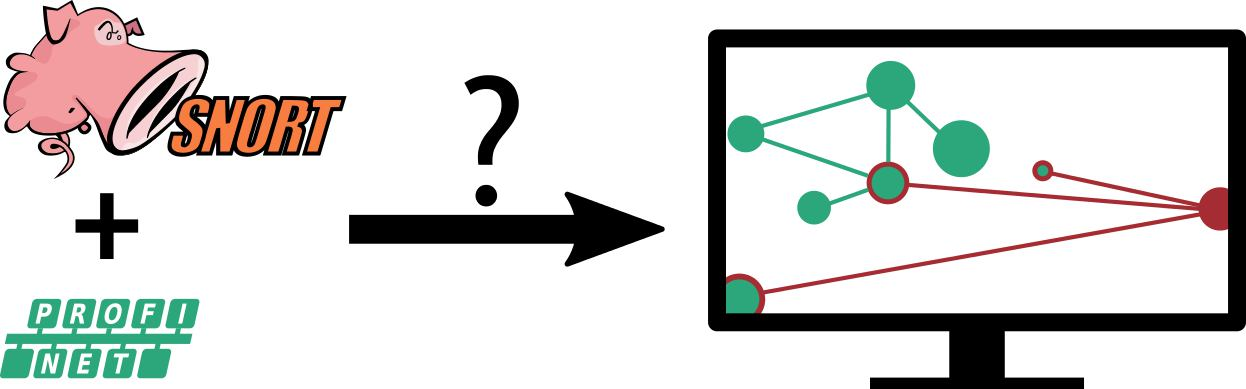
\includegraphics[width=\textwidth]{./images/aufgabestellung.jpg}
  \caption{Aufgabe visualisiert}
\end{figure}
\end{frame}